\documentclass[a4paper,11pt]{article}

\usepackage[ansinew]{inputenc}
\usepackage[french]{babel}
\usepackage[T1]{fontenc}
\usepackage[paper=a4paper, top=1cm, bottom=1cm, left=2cm, right=2cm]{geometry}
\usepackage{graphicx}
\usepackage{hyperref}
\usepackage{url}
\usepackage{xcolor}

\title{Legend Of Zelda}
\author{Beno�t V�drenne, Ga�l Walter}

\begin{document}

\maketitle

\begin{abstract}
Dans The Legend of Zelda, le joueur incarne un jeune gar�on, parfois un jeune homme, nomm� Link et doit, arm� de son �p�e et de son bouclier, sauver la princesse Zelda. (WikiPedia !)
\end{abstract}

\begin{center}
 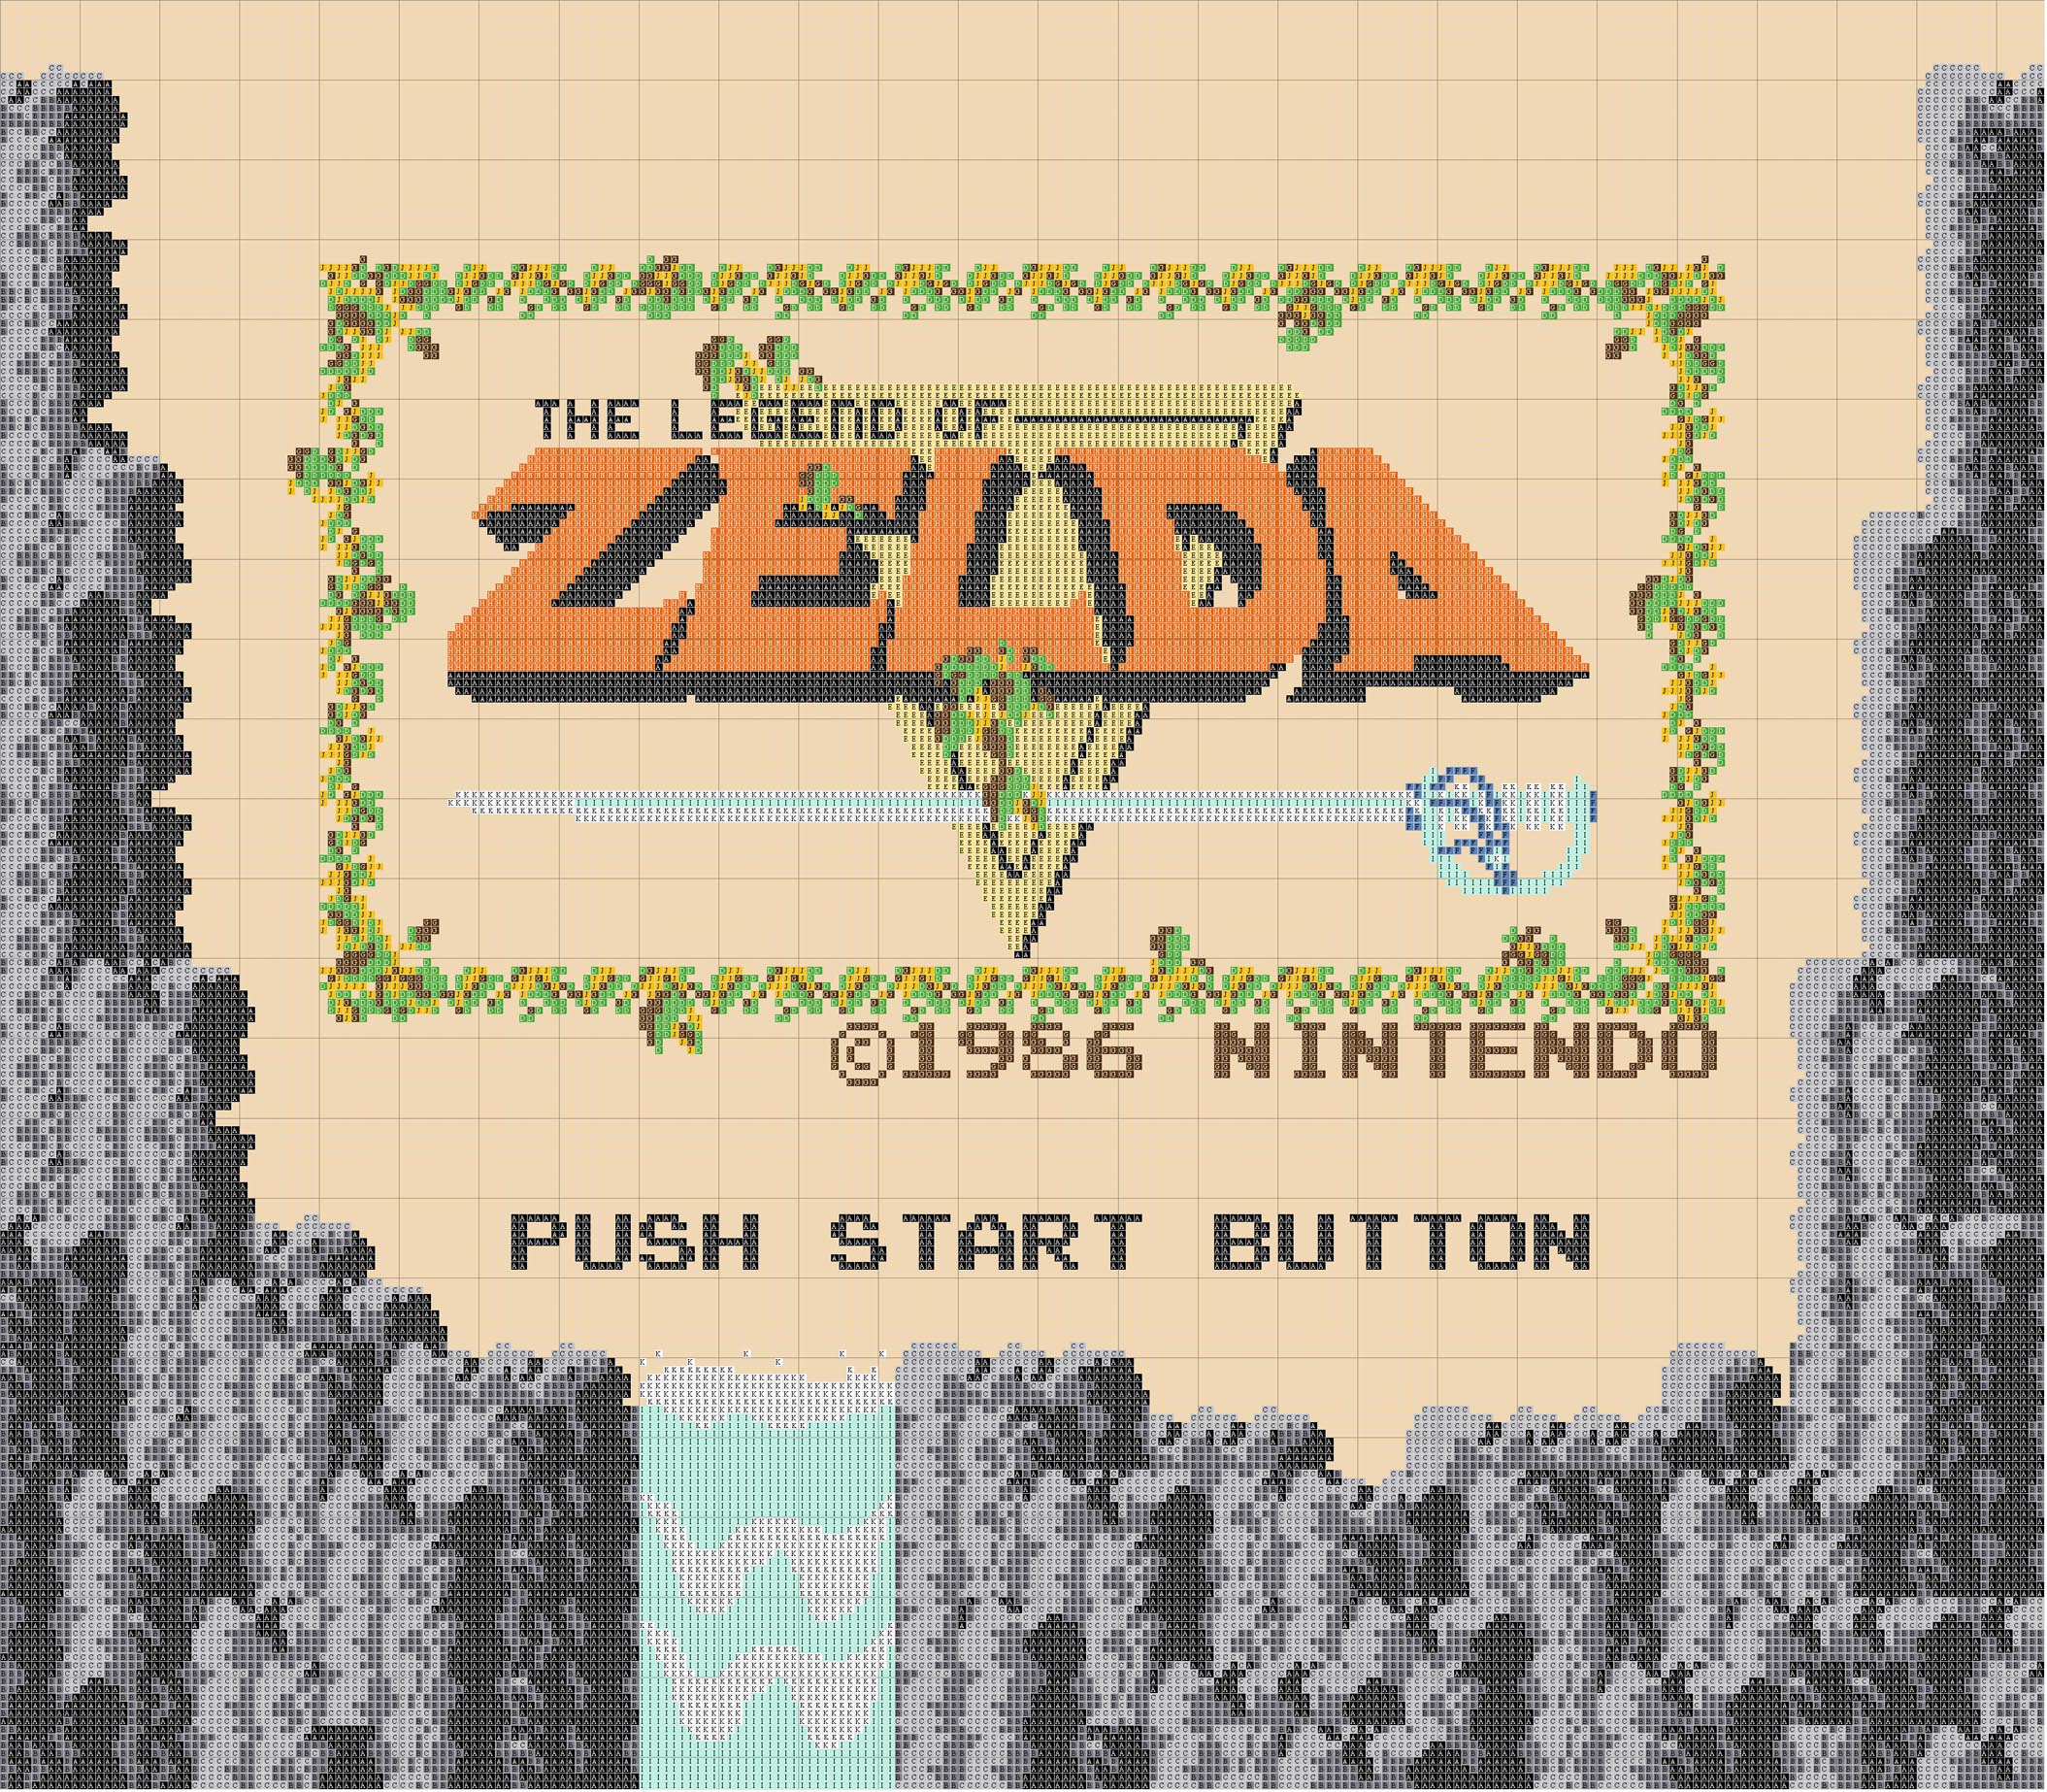
\includegraphics[width=9cm,height=7cm]{images/zeldaNintendo.eps}
\end{center}

\section{Introduction}
\section{Jouer � Zelda-VW}
\section{D�veloppement}
\section{Conclusion}

\end{document}
